\chapter*{General Introduction}
\graphicspath{{Introduction/figures/}}
\addcontentsline{toc}{chapter}{General Introduction}
\begin{spacing}{1.2}
%==================================================================================================%

In the modern software world APIs are becoming a must for every tech company to allow products to be integrated by developers in multiple Apps.

APIs do all this by "exposing" some of a product's internal functions to the outside world in a limited fashion. That makes it possible for applications to share data and take actions on one another's behalf without requiring developers to share all of their software's code. 



\begin{figure}[!ht]\centering
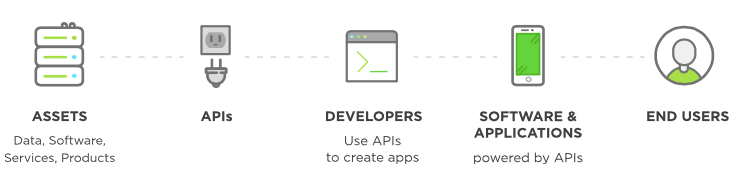
\includegraphics[scale=0.6]{API.png}
\caption{APIs }
\label{fig:fig1}
\end{figure}

That's the reason why KAOUN, a Tunisian FinTech start-up, decided to create its own developers API for its main product FLOUCI which is a mobile payment solution. This project will expand FLOUCI to the developers world and unleash the full potential of the product, also it could take FLOUCI into new markets and open doors for unlimited integrations.\newline


The following report is a synthesis of the efforts done to build FLOUCI developers API.

 To detail the process of our work, we have divided this report into XX chapters representing the different aspects of our project.

In the first chapter, entitled Project scope, we started with a presentation of the host company. Afterwards, we gave an overview of our project and we detailed the followed methodology for its realization.


The second chapter is about the development disciplines and rules we set during our project development life cycle. It's a detailed explanation of the development practices needed to start our project development in the most efficient way possible. 



We close our work with a general conclusion in which we try to evaluate our contribution as well as we develop our vision for the project's potential improvements.




\end{spacing}
